%==============================================================================
%  BVH Raytracer -- Diapositivas (tema oscuro + naranja, UTEC)
%  Compilar con:  xelatex slides.tex   (2 pasadas)
%==============================================================================
% !TEX program = xelatex
\documentclass[aspectratio=169,11pt]{beamer}

% --- Tipografia (xelatex + fuentes del sistema, con fallback seguro) ---
\usepackage{fontspec}
\IfFontExistsTF{Optima}{\setsansfont{Optima}}{\IfFontExistsTF{Gill Sans}{\setsansfont{Gill Sans}}{}}
\IfFontExistsTF{Menlo}{\setmonofont{Menlo}[Scale=0.82]}{}
\renewcommand{\familydefault}{\sfdefault}

% --- Idioma ---
\usepackage[spanish,es-noshorthands]{babel}

% --- Paquetes ---
\usepackage{amsmath,amssymb}
\usepackage{graphicx}
\usepackage{booktabs}
\usepackage{array}
\usepackage{colortbl}
\usepackage{xcolor}
\usepackage{tikz}
\usetikzlibrary{positioning,arrows.meta,calc,shapes.geometric,fit}
\usepackage{listings}

%==============================================================================
%   PALETA  (fondo CLARO + texto negro oscuro + naranja principal)
%==============================================================================
\definecolor{bg}{HTML}{FFFFFF}        % fondo blanco
\definecolor{panel}{HTML}{F0F2F5}     % paneles / bloques (gris claro)
\definecolor{panellt}{HTML}{E4E8EC}   % panel un poco mas oscuro
\definecolor{ink}{HTML}{161B22}       % TEXTO negro oscuro (alto contraste)
\definecolor{mute}{HTML}{5C6570}      % gris secundario legible
\definecolor{rule}{HTML}{D8DCE0}      % lineas tenues
\definecolor{prim}{HTML}{F58220}      % NARANJA principal
\definecolor{primdk}{HTML}{C75A0C}    % naranja oscuro (para texto sobre blanco)
\definecolor{primlt}{HTML}{FFD9A8}    % naranja muy claro (fondos suaves)

%==============================================================================
%   TEMA OSCURO PROPIO
%==============================================================================
\usefonttheme{professionalfonts}
\setbeamertemplate{navigation symbols}{}
\setbeamersize{text margin left=11mm, text margin right=11mm}

\setbeamercolor{background canvas}{bg=bg}
\setbeamercolor{normal text}{fg=ink}
\setbeamercolor{structure}{fg=primdk}
\setbeamercolor{alerted text}{fg=primdk}
\setbeamercolor{example text}{fg=primdk}
\setbeamercolor{title}{fg=primdk}
\setbeamercolor{subtitle}{fg=mute}
\setbeamercolor{author}{fg=ink}
\setbeamercolor{date}{fg=mute}
\setbeamercolor{institute}{fg=mute}
\setbeamercolor{itemize item}{fg=prim}
\setbeamercolor{itemize subitem}{fg=primdk}
\setbeamercolor{section in toc}{fg=ink}
\setbeamercolor{section number projected}{bg=prim,fg=white}
\setbeamercolor{block title}{fg=white,bg=prim}
\setbeamercolor{block body}{fg=ink,bg=panel}
\setbeamercolor{block title alerted}{fg=white,bg=primdk}
\setbeamercolor{block body alerted}{fg=ink,bg=panel}
\setbeamercolor{block title example}{fg=ink,bg=primlt}
\setbeamercolor{block body example}{fg=ink,bg=panel}

\setbeamerfont{frametitle}{series=\bfseries,size=\Large}
\setbeamerfont{title}{series=\bfseries,size=\LARGE}
\setbeamerfont{footer}{size=\scriptsize}

\setbeamertemplate{itemize item}{\small\raise1.2pt\hbox{\textcolor{prim}{$\blacktriangleright$}}}
\setbeamertemplate{itemize subitem}{\textcolor{primlt}{\textbullet}}

% Frame title: naranja + filete (versión robusta, sin overfull)
\setbeamertemplate{frametitle}{%
  \nointerlineskip
  \begin{beamercolorbox}[wd=\paperwidth,leftskip=11mm,rightskip=11mm,ht=3.4ex,dp=1.4ex]{}
    \usebeamerfont{frametitle}\color{primdk}\insertframetitle
  \end{beamercolorbox}%
  \vskip1pt\hspace*{11mm}{\color{primdk}\rule{\dimexpr\paperwidth-22mm\relax}{1.4pt}}\vskip4pt%
}

% Footer
\setbeamertemplate{footline}{%
  \leavevmode\hbox{%
    \begin{beamercolorbox}[wd=.62\paperwidth,ht=2.6ex,dp=1.4ex,leftskip=11mm]{footer}%
      \color{mute}\insertshorttitle
    \end{beamercolorbox}%
    \begin{beamercolorbox}[wd=.38\paperwidth,ht=2.6ex,dp=1.4ex,rightskip=11mm]{footer}%
      \hfill\color{mute}\insertframenumber\,{\color{rule}|}\,\inserttotalframenumber
    \end{beamercolorbox}}%
  \vspace{2pt}%
}

% Slide de seccion
\AtBeginSection[]{%
  \begin{frame}[plain,noframenumbering]
    \vfill\centering
    {\color{mute}\footnotesize\bfseries SECCI\'ON \insertsectionnumber}\\[6pt]
    {\color{primdk}\Huge\bfseries \insertsectionhead}\\[10pt]
    {\color{primdk}\rule{0.28\textwidth}{1.6pt}}
    \vfill
  \end{frame}
}

%==============================================================================
%   LISTINGS (estilo oscuro)
%==============================================================================
\lstdefinestyle{cppx}{
  language=C++,
  basicstyle=\ttfamily\scriptsize\color{ink},
  keywordstyle=\color{primdk}\bfseries,
  commentstyle=\color{mute}\itshape,
  stringstyle=\color{A05A1C},
  showstringspaces=false, breaklines=true,
  frame=leftline, framerule=1.4pt, rulecolor=\color{primdk},
  backgroundcolor=\color{panel},
  xleftmargin=8pt, tabsize=2,
  morekeywords={vec3,vec4,AABB,Tri,Hit,Node,uint32_t,std,nullptr,constexpr,auto}
}
\lstset{style=cppx}

\graphicspath{{./}}
\newcommand{\vecm}[1]{\mathbf{#1}}
\newcommand{\hl}[1]{{\color{primdk}\textbf{#1}}}

\arrayrulecolor{rule}

%==============================================================================
\title[Ray tracing con BVH]{Ray tracing acelerado con BVH}
\author{Kalos Lazo \and Marcelo Chincha \and Lenin Ch\'avez}
\date{\today}

\begin{document}

%========================== PORTADA ===========================================
\begin{frame}[plain,noframenumbering]
\begin{tikzpicture}[remember picture,overlay]
  \fill[prim] (current page.north west) rectangle ([yshift=-6mm]current page.north east);
  \fill[bg]   ([yshift=-6mm]current page.north west) rectangle ([yshift=-7mm]current page.north east);
  \fill[prim] ([yshift=-7mm]current page.north west) rectangle ([yshift=-8mm]current page.north east);
  \fill[prim] (current page.south west) rectangle ([yshift=4mm]current page.south east);
\end{tikzpicture}

\vspace{18mm}
\begin{center}
{\color{mute}\footnotesize\bfseries PROYECTO FINAL \textbullet{} CS3014 \textbullet{} UTEC}\\[14pt]
{\color{primdk}\Huge\bfseries Ray tracing acelerado con BVH}\\[12pt]
{\color{primdk}\rule{0.4\textwidth}{1.4pt}}\\[12pt]
{\color{ink}\large Estudio comparativo de heur\'isticas de construcci\'on}\\[3pt]
{\color{mute}\normalsize SAH \textbullet{} Median \textbullet{} Morton \textbullet{} Intel Embree}
\end{center}

\vfill
\begin{center}
\color{ink}\small\bfseries Kalos Lazo \quad\textbullet\quad Marcelo Chincha \quad\textbullet\quad Lenin Ch\'avez\\[3pt]
\color{mute}\footnotesize Universidad de Ingenier\'ia y Tecnolog\'ia \textbullet{} 2026-1
\end{center}
\end{frame}

%========================== AGENDA ============================================
\begin{frame}{Agenda}
\setbeamertemplate{section in toc}[sections numbered]
\setbeamerfont{section in toc}{size=\small}
\begin{columns}[T]
\begin{column}{0.5\textwidth}
\tableofcontents[sections={1-5}]
\end{column}
\begin{column}{0.5\textwidth}
\tableofcontents[sections={6-9}]
\end{column}
\end{columns}
\end{frame}

%==============================================================================
\section{Introducci\'on}
%==============================================================================

\begin{frame}{¿Qu\'e es el ray tracing?}
\begin{columns}[T]
\begin{column}{0.58\textwidth}
\begin{itemize}\itemsep5pt
  \item T\'ecnica de renderizado que \hl{simula el camino de la luz}: por cada
        p\'ixel se lanza un \emph{rayo} desde la c\'amara.
  \item El rayo \hl{rebota}, genera \hl{sombras} y \hl{reflejos} siguiendo
        leyes \'opticas $\Rightarrow$ imagen fotorrealista.
  \item Es el est\'andar en cine de animaci\'on y, hoy, tambi\'en en
        videojuegos (\emph{NVIDIA RTX}, PS5).
\end{itemize}
\end{column}
\begin{column}{0.42\textwidth}\centering
\begin{tikzpicture}[scale=0.85,every node/.style={font=\scriptsize,text=ink}]
  \draw[->,thick,primlt] (-0.2,0) -- (4.8,0.7) node[midway,above]{rayo};
  \node[draw=primlt,fill=panellt,minimum width=1.3cm,minimum height=0.9cm] (a) at (4.8,0.7){};
  \draw[->,thick,prim] (4.8,0.7) -- (3.0,2.4) node[midway,right]{reflejo};
  \node[draw=prim,fill=panellt,circle,minimum size=0.5cm] at (2.8,2.6){};
  \node[mute] at (4.8,-0.3) {espejo};
  \node[mute] at (0,-0.3) {c\'amara};
\end{tikzpicture}
\end{column}
\end{columns}
\end{frame}

\begin{frame}{¿Por qu\'e importa?}
\begin{block}{D\'onde se usa hoy el ray tracing}
\begin{itemize}\itemsep2pt
  \item \hl{Cine / animaci\'on:} Pixar, Disney, ILM (toda pel\'icula CG moderna).
  \item \hl{Videojuegos:} \emph{Cyberpunk 2077}, \emph{Minecraft RTX} \textemdash{} iluminaci\'on global en tiempo real.
  \item \hl{Dise\~no y arquitectura:} previsualizaci\'on fotorrealista.
  \item \hl{Ciencia e IA:} radar, simulaci\'on, \emph{neural rendering}.
\end{itemize}
\end{block}
\vspace{3pt}
\begin{alertblock}{El reto}
Es \hl{computacionalmente muy caro}. Su viabilidad depende de \emph{estructuras de
datos} que lo aceleren $\rightarrow$ \hl{el BVH}.
\end{alertblock}
\end{frame}

%==============================================================================
\section{Nuestro enfoque}
%==============================================================================

\begin{frame}{Nuestro enfoque}
\begin{columns}[T]
\begin{column}{0.52\textwidth}
\begin{itemize}\itemsep4pt
  \item Ray tracer \hl{por software en CPU}, multihilo (4+ workers).
  \item Aceleraci\'on: \hl{BVH propio} con SAH / Median / Morton (seleccionable en vivo).
  \item \hl{Dos BVH} (est\'atico + din\'amico) \textemdash{} ver siguiente.
  \item Sombras, reflejos recursivos, iluminaci\'on indirecta (NEE).
  \item Backend \hl{GPU OpenCL} opcional.
  \item Referencia industrial: \hl{Intel Embree 4}.
\end{itemize}
\end{column}
\begin{column}{0.48\textwidth}\centering
\begin{tikzpicture}[scale=0.62,every node/.style={font=\scriptsize,text=ink},
  b/.style={draw=prim,thick,rounded corners=2pt,fill=panel,minimum width=2.5cm,minimum height=0.6cm},
  a/.style={-Stealth,thick,primlt}]
  \node[b] (app) at (0,4) {App / c\'amara};
  \node[b] (acc) at (0,2.8) {Aceleraci\'on (BVH)};
  \node[b] (sh)  at (0,1.6) {Sombreado};
  \node[b] (gpu) at (3.6,2.8) {GPU (OpenCL)};
  \node[b] (emb) at (3.6,4) {Embree (ref.)};
  \draw[a] (app)--(acc); \draw[a] (acc)--(sh);
  \draw[a,dashed] (acc)--(gpu); \draw[a,dashed] (app)--(emb);
\end{tikzpicture}
\end{column}
\end{columns}
\end{frame}

\begin{frame}{Dos BVH: est\'atico + din\'amico}
\begin{columns}[T]
\begin{column}{0.5\textwidth}
\begin{block}{BVH est\'atico \textemdash{} \textcolor{primlt}{SAH}}
\begin{itemize}\itemsep2pt
  \item Contiene la \hl{escena fija} (edificios, calles).
  \item Se construye \hl{una sola vez} con SAH (mejor calidad).
  \item Se reutiliza en todos los frames.
\end{itemize}
\end{block}
\end{column}
\begin{column}{0.5\textwidth}
\begin{exampleblock}{BVH din\'amico \textemdash{} \textcolor{primlt}{Morton}}
\begin{itemize}\itemsep2pt
  \item Objetos que \hl{se mueven} (peatreros/peatones, meshes).
  \item Se \hl{reconstruye cada frame} $\Rightarrow$ Morton (build rapid\'isimo).
  \item Pocos tri\'angulos $\Rightarrow$ calidad suficiente.
\end{itemize}
\end{exampleblock}
\end{column}
\end{columns}
\vspace{4pt}
\centering\small Cada rayo consulta \hl{ambos} \'arboles y se queda con el golpe m\'as cercano.\\[2pt]
\footnotesize\textcolor{mute}{Idea clave: la heur\'istica debe casar con la frecuencia de cambio de la geometr\'ia.}
\end{frame}

%==============================================================================
\section{El problema y la idea}
%==============================================================================

\begin{frame}{El problema: el ray tracing ingenuo es intratable}
El rayo se prueba contra \hl{todos} los tri\'angulos:
\[
T_{\text{frame}} \;\approx\; \underbrace{P}_{\text{p\'ixeles}}\cdot
\underbrace{N}_{\text{tri\'angulos}}\cdot(\text{rayos secundarios})
\]
\begin{alertblock}{Un n\'umero que asusta}
$1280\times720$ con $50\,000$ tri\'angulos $\approx 4{,}6\times10^{10}$ tests por
frame $\Rightarrow$ \hl{$\sim$46\,s por frame}. Imposible en tiempo real.
\end{alertblock}
\begin{itemize}
  \item Necesitamos \hl{descartar} grandes grupos de tri\'angulos con pruebas baratas.
  \item $\Rightarrow$ una estructura de aceleraci\'on: el \alert{BVH}.
\end{itemize}
\end{frame}

\begin{frame}{BVH: la idea}
\begin{columns}[T]
\begin{column}{0.54\textwidth}
\begin{itemize}\itemsep3pt
  \item \'Arbol binario de \hl{cajas alineadas a los ejes} (AABB).
  \item La ra\'iz envuelve toda la escena; cada nodo \hl{parte} sus tri\'angulos en 2 hijos.
  \item Las \hl{hojas} guardan pocos tri\'angulos.
  \item El rayo prueba primero las cajas y solo desciende por las que golpea.
\end{itemize}
\end{column}
\begin{column}{0.46\textwidth}\centering
\begin{tikzpicture}[scale=0.72,every node/.style={font=\scriptsize,text=ink},
  bx/.style={draw=prim,thick,rounded corners=1pt,fill=panel},
  lf/.style={draw=primlt,thick,rounded corners=1pt,fill=panellt},
  e/.style={-Stealth,thick,primlt}]
  \node[bx,minimum width=2.6cm,minimum height=0.45cm] (r) at (0,3) {ra\'iz};
  \node[bx,minimum width=1.6cm,minimum height=0.4cm] (a) at (-1.8,1.7) {hijo izq.};
  \node[bx,minimum width=1.6cm,minimum height=0.4cm] (b) at (1.8,1.7) {hijo der.};
  \node[lf] (l1) at (-2.6,0.3) {hoja};
  \node[lf] (l2) at (-1.0,0.3) {hoja};
  \node[lf] (l3) at (1.0,0.3) {hoja};
  \node[lf] (l4) at (2.6,0.3) {hoja};
  \draw[e] (r)--(a); \draw[e] (r)--(b);
  \draw[e] (a)--(l1); \draw[e] (a)--(l2);
  \draw[e] (b)--(l3); \draw[e] (b)--(l4);
\end{tikzpicture}
\end{column}
\end{columns}
\vspace{4pt}
\centering Costo por rayo: $O(N)\;\to\;\sim$\hl{$O(\log N)$}.
\end{frame}

%==============================================================================
\section{Conceptos clave}
%==============================================================================

\begin{frame}{AABB y el test de los \emph{slabs}}
\begin{columns}[T]
\begin{column}{0.56\textwidth}
\small
\textbf{AABB}: caja alineada a los ejes, con 2 esquinas (\texttt{min}, \texttt{max}).\\[2pt]
\textbf{Slab}: banda entre 2 planos paralelos; una caja $=$ 3 slabs (X, Y, Z).\\[2pt]
El rayo entra en los 3 slabs a la vez sii:
\vspace{-2pt}
\[
t_{\min}\!=\!\max(\text{ent.})\le t_{\max}\!=\!\min(\text{sal.})\;\Rightarrow\;\hl{\text{golpea}}
\]
\end{column}
\begin{column}{0.44\textwidth}\centering
\begin{tikzpicture}[scale=0.56,every node/.style={font=\scriptsize,text=ink}]
  \fill[panel] (0,0) rectangle (4,2.5);
  \draw[thick,prim] (0,0) rectangle (4,2.5);
  \draw[dashed,mute] (0,-0.5)--(0,3); \draw[dashed,mute] (4,-0.5)--(4,3);
  \draw[->,very thick,primlt] (-1.2,1.0)--(4.6,1.5) node[right]{rayo};
  \node[prim] at (2,2.75) {AABB};
\end{tikzpicture}
\end{column}
\end{columns}
\begin{exampleblock}{Optimizaci\'on clave}
Se precalcula $\mathrm{inv}=1/\vecm{D}$ por rayo $\Rightarrow$ luego solo se multiplica (divisi\'on $\sim$20$\times$ m\'as lenta).
\end{exampleblock}
\end{frame}

\begin{frame}[fragile]{M\"oller\textendash Trumbore: rayo\,--\,tri\'angulo}
Iguala el rayo $\vecm{P}=\vecm{O}+t\vecm{D}$ con el tri\'angulo
$\vecm{P}=\vecm{v_0}+u\,\vecm{e_1}+v\,\vecm{e_2}$ y resuelve $(t,u,v)$:
\begin{lstlisting}
vec3 e1 = v1 - v0, e2 = v2 - v0;
vec3 h  = cross(d, e2);
float a = dot(e1, h);                 if (fabs(a) < EPS) return false;
float f = 1.0f / a;
float u = f * dot(o - v0, h);         if (u < 0 || u > 1) return false;
float v = f * dot(d, cross(o-v0,e1)); if (v < 0 || u+v > 1) return false;
t = f * dot(e2, cross(o-v0, e1));     return t > EPS;
\end{lstlisting}
\vspace{2pt}
\small $u,v\ge0$ y $u{+}v\le1$ \emph{son} la prueba de \emph{dentro del tri\'angulo}; adem\'as
$(u,v)$ son los \alert{pesos baric\'entricos} para interpolar color, normal y textura.
\end{frame}

%==============================================================================
\section{Construcci\'on del \'arbol}
%==============================================================================

\begin{frame}{Construcci\'on \emph{top-down}}
\begin{enumerate}\itemsep3pt
  \item Se parte con \hl{todos} los tri\'angulos en la ra\'iz.
  \item Centroide de cada uno: $(v_0+v_1+v_2)/3$.
  \item Mientras un nodo tenga $>2$ tri\'angulos:
    \begin{itemize}
      \item eje de mayor extensi\'on de centroides;
      \item plano de corte $\Rightarrow$ \emph{depende de la heur\'istica};
      \item reparto por centroide en 2 hijos.
    \end{itemize}
  \item Recursi\'on hasta hojas de $\le 2$ tri\'angulos.
\end{enumerate}
\vspace{3pt}
\begin{block}{La pregunta del proyecto}
¿\hl{D\'onde} cortar? Comparamos 3 heur\'isticas \textemdash{} y de eso vive el \emph{benchmark}.
\end{block}
\end{frame}

\begin{frame}{Tres heur\'isticas de construcci\'on}
\begin{columns}[T]
\begin{column}{0.33\textwidth}
\begin{block}{SAH\hfill\textcolor{primlt}{$\bigstar$}}
Minimiza el \hl{costo} = \'area $\times$ n.$^\circ$ de tri\'angulos. 12 cubos (\emph{binning}).
\\[2pt]\footnotesize\textcolor{mute}{Mejor \'arbol; build m\'as lento.}
\end{block}
\end{column}
\begin{column}{0.33\textwidth}
\begin{exampleblock}{Median}
Corta por la \hl{mediana} de centroides (mitad/mitad).
\\[2pt]\footnotesize\textcolor{mute}{Simple; ignora el tama\~no.}
\end{exampleblock}
\end{column}
\begin{column}{0.33\textwidth}
\begin{block}{Morton}
Ordena por \hl{c\'odigo Z} (bits intercalados) y corta por la mitad del \'indice.
\\[2pt]\footnotesize\textcolor{mute}{Build rapid\'isimo; \'arbol mediocre.}
\end{block}
\end{column}
\end{columns}
\vspace{5pt}
\centering Comparten centroides, eje y recursi\'on; solo cambia \alert{d\'onde cortar}.
\end{frame}

\begin{frame}{SAH: heur\'istica de \'area de superficie}
\textbf{Intuici\'on:} un rayo es m\'as probable de entrar en una caja m\'as grande.
$P(\text{entrar en hijo})\propto$ \'area(hijo)/\'area(padre). Costo esperado:
\[
C_{\text{split}} = 1 + \frac{A_L\,n_L + A_R\,n_R}{A_{\text{padre}}}
\]
\begin{columns}[T]
\begin{column}{0.52\textwidth}
\textbf{Binning}: en vez de probar todos los cortes $O(N^2)$, se dividen los centroides en
\alert{12 cubos} y se prueban solo 11 cortes $\Rightarrow$ build $O(N\log N)$, casi \'optimo.
\end{column}
\begin{column}{0.48\textwidth}\centering
\begin{tikzpicture}[scale=0.62,every node/.style={font=\scriptsize,text=ink}]
  \foreach \i in {0,...,11}{\draw[rule,fill=panel] (\i*0.5,0) rectangle (\i*0.5+0.5,0.7);}
  \foreach \i/\h in {1/0.5,2/0.6,3/0.35,7/0.2,8/0.55,9/0.65,10/0.45}{
    \fill[prim] (\i*0.5,0) rectangle (\i*0.5+0.5,\h);}
  \draw[thick,primlt,dashed] (3.5,-0.1)--(3.5,0.95);
  \node[primlt] at (3.5,1.15) {\scriptsize corte};
\end{tikzpicture}
\end{column}
\end{columns}
\end{frame}

%==============================================================================
\section{Recorrido y pipeline}
%==============================================================================

\begin{frame}[fragile]{Recorrido (\emph{traversal}) con pila y poda}
\begin{columns}[T]
\begin{column}{0.5\textwidth}
\begin{itemize}\itemsep2pt
  \item Recorrido \hl{iterativo} con pila fija (no recursi\'on).
  \item \hl{Poda 1:} caja no golpeada $\Rightarrow$ se salta el sub\'arbol.
  \item \hl{Poda 2:} caja m\'as lejos que el mejor $t$ $\Rightarrow$ se salta.
  \item En la hoja: M\"oller\textendash Trumbore a sus pocos tri\'angulos.
\end{itemize}
\end{column}
\begin{column}{0.5\textwidth}
\begin{lstlisting}
stack.push(raiz);
while (pila no vacia) {
  nodo = pop();
  if (!aabb_hit(nodo.box, inv, best)) continue;  // poda
  if (es_hoja)  test_tris(nodo);
  else          push(hijos);
}
\end{lstlisting}
\end{column}
\end{columns}
\vspace{2pt}
\centering\small Un rayo que tocar\'ia miles de tri\'angulos acaba probando \alert{solo unos pocos}.
\end{frame}

\begin{frame}{Pipeline completo}
\centering
\begin{tikzpicture}[
  node distance=3mm and 4mm,
  box/.style={draw=prim,thick,rounded corners=2pt,fill=panel,
              minimum width=2.2cm,minimum height=0.8cm,align=center,font=\scriptsize,text=ink},
  fin/.style={draw=primlt,thick,rounded corners=2pt,fill=panellt,
              minimum width=2.2cm,minimum height=0.8cm,align=center,font=\scriptsize\bfseries,text=ink},
  arr/.style={-Stealth,thick,primlt}]
  \node[box] (cam) {C\'amara\\+ rayo};
  \node[box,right=of cam] (bvh) {Recorrido\\BVH};
  \node[box,right=of bvh] (hit) {Golpe\\$(t,u,v)$};
  \node[box,right=of hit] (sh) {Sombreado\\luz + sombra};
  \node[fin,right=of sh] (px) {Color\\del p\'ixel};
  \draw[arr] (cam)--(bvh); \draw[arr] (bvh)--(hit);
  \draw[arr] (hit)--(sh);  \draw[arr] (sh)--(px);
  \draw[arr] (sh.south) -- ++(0,-0.55) -| node[below,pos=0.25,font=\tiny\itshape,prim]{reflejo (recursi\'on)} (bvh.south);
\end{tikzpicture}
\vspace{8pt}
\begin{itemize}
  \item El sombreado puede \hl{generar nuevos rayos} (sombra, reflejo) $\Rightarrow$ recursi\'on.
  \item La imagen se reparte en \alert{franjas} entre los n\'ucleos (multihilo, sem\'aforos SDL).
\end{itemize}
\end{frame}

%==============================================================================
\section{Complejidades}
%==============================================================================

\begin{frame}{Complejidades del BVH}
\begin{table}\centering\small
\renewcommand{\arraystretch}{1.25}
\begin{tabular}{lll}
\toprule
\textbf{Operaci\'on} & \textbf{Complejidad} & \textbf{Nota} \\
\midrule
Build \hl{SAH} (binning)   & $O(N\log N)$ & 12 cubos por nodo, casi \'optimo \\
Build \textcolor{primlt}{Morton}        & $O(N\log N)$ & domina el \emph{sort} \\
Build Median               & $O(N\log N)$ & quickselect $O(N)$ por nivel \\
\rowcolor{panellt}
\textbf{Recorrido} (promedio) & $\boldsymbol{O(\log N)}$ & descarta sub\'arboles \\
Recorrido (peor caso)      & $O(N)$       & geometr\'ia degenerada \\
Memoria                    & $O(N)$       & nodos + tri\'angulos \\
Rayo\,--\,AABB (slab)      & $O(1)$       & 3 ejes \\
Rayo\,--\,tri\'angulo      & $O(1)$       & M\"oller\textendash Trumbore \\
\bottomrule
\end{tabular}
\end{table}
\vspace{4pt}
\centering\footnotesize\textcolor{mute}{$N$ = n.$^\circ$ de tri\'angulos. La calidad del \'arbol cambia la \emph{constante} del recorrido, no la asint\'otica.}
\end{frame}

%==============================================================================
\section{Resultados}
%==============================================================================

\begin{frame}{Setup experimental}
\begin{columns}[T]
\begin{column}{0.5\textwidth}
\textbf{Escena:} ciudad procedural (fachadas con ventanas):
\begin{itemize}\itemsep1pt
  \item Small: \hl{14\,896} tri\'angulos
  \item Medium: \hl{18\,468}
  \item Large: \hl{31\,644}
\end{itemize}
\textbf{Plataforma:} Apple M5, 10 n\'ucleos (4P+6E), \texttt{-O3 -march=native}.\\[2pt]
\textbf{Referencia:} \alert{Intel Embree 4} sobre la misma geometr\'ia.
\end{column}
\begin{column}{0.5\textwidth}
\textbf{Metodolog\'ia} (reproducible: \texttt{-{}-bench}):
\begin{itemize}\itemsep1pt
  \item 5 frames de \emph{warmup} $+$ promedio de 20.
  \item Traversal puro (1 hilo, sin sombreado).
  \item \alert{Nodos/rayo}: visitas por rayo \textemdash{} m\'etrica hardware-independiente.
\end{itemize}
\end{column}
\end{columns}
\end{frame}

\begin{frame}{Resultado principal \textemdash{} escena Large (31\,644 tri\'angulos)}
\begin{table}\centering\small
\setlength{\tabcolsep}{7pt}
\renewcommand{\arraystretch}{1.2}
\begin{tabular}{lrrrr}
\toprule
\textbf{Estrategia} & \textbf{Build (ms)} & \textbf{Render (ms)} & \textbf{Trav. (ms)} & \textbf{Nodos/rayo} \\
\midrule
\hl{SAH (nuestra)}      & 6{,}4 & \hl{112} & \hl{79}  & \hl{367}  \\
Median                  & 5{,}0 & 199       & 151       & 701        \\
Morton                  & \hl{2{,}6} & 288   & 242       & 1\,119     \\
\midrule
\rowcolor{panellt}
\textcolor{primlt}{\textbf{Embree}} (referencia) & --- & --- & \textcolor{primlt}{\textbf{33}} & --- \\
\bottomrule
\end{tabular}
\end{table}
\vspace{4pt}
\begin{itemize}\itemsep2pt
  \item SAH visita \hl{$\sim$3$\times$ menos nodos} que Morton $\Rightarrow$ render \hl{$\sim$2{,}6$\times$ m\'as r\'apido}.
  \item Embree recorre $\sim$2{,}4$\times$ m\'as r\'apido que nuestra SAH (kernels SIMD).
\end{itemize}
\end{frame}

\begin{frame}{Calidad del \'arbol: SAH domina}
\begin{columns}[T]
\begin{column}{0.6\textwidth}\centering
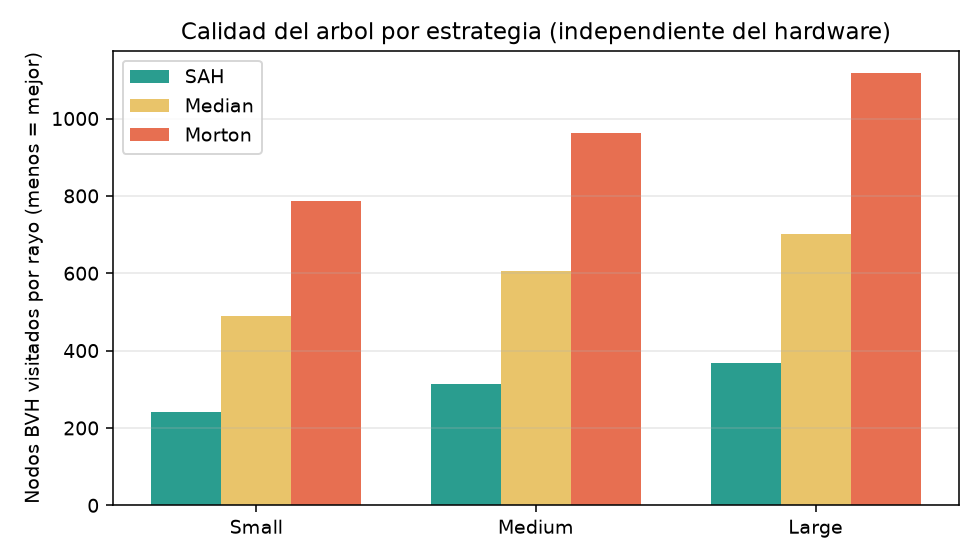
\includegraphics[width=\textwidth,height=0.72\textheight,keepaspectratio]{fig_quality.png}
\end{column}
\begin{column}{0.4\textwidth}
\begin{itemize}\itemsep3pt
  \item M\'etrica \alert{nodos/rayo}: independiente del hardware.
  \item SAH es la m\'as baja \emph{en todas las densidades}.
  \item En Large: \hl{SAH 367 vs Morton 1\,119}.
\end{itemize}
\end{column}
\end{columns}
\end{frame}

\begin{frame}{Compromiso \emph{build} vs calidad}
\begin{columns}[T]
\begin{column}{0.6\textwidth}\centering
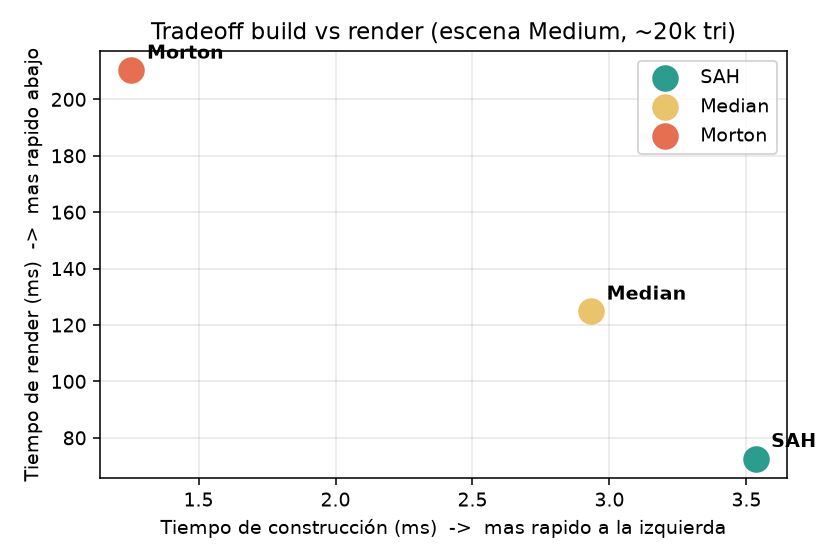
\includegraphics[width=\textwidth,height=0.72\textheight,keepaspectratio]{fig_tradeoff.png}
\end{column}
\begin{column}{0.4\textwidth}
\begin{itemize}\itemsep2pt
  \item Esquina abajo-izquierda $=$ ideal.
  \item Morton: build r\'apido, render lento.
  \item SAH: build m\'as lento, render mucho m\'as r\'apido.
  \item Se construye \emph{1 vez} y se recorre \emph{millones} $\Rightarrow$ \alert{compensa SAH}.
\end{itemize}
\end{column}
\end{columns}
\end{frame}

\begin{frame}{Escalado con el tama\~no de escena}
\begin{columns}[T]
\begin{column}{0.6\textwidth}\centering
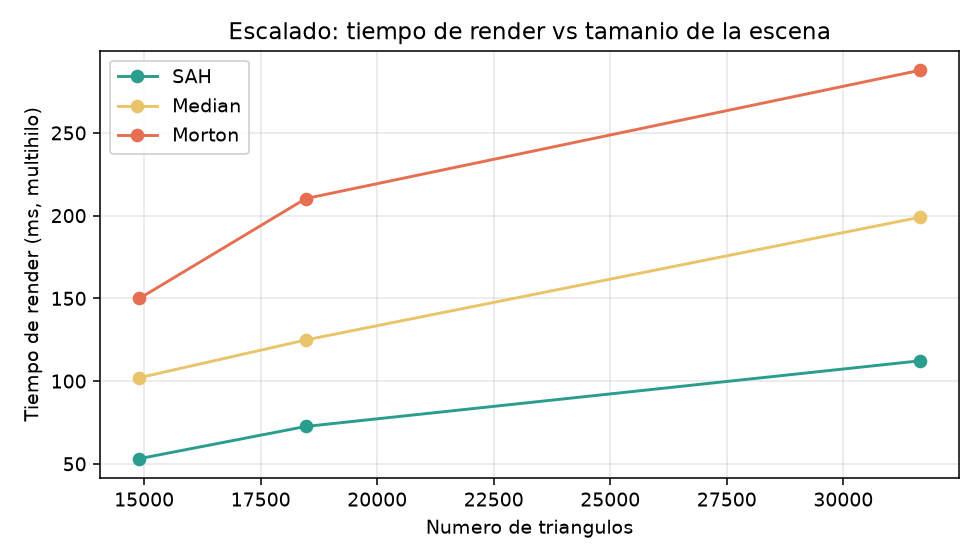
\includegraphics[width=\textwidth,height=0.72\textheight,keepaspectratio]{fig_scaling.png}
\end{column}
\begin{column}{0.4\textwidth}
\begin{itemize}\itemsep2pt
  \item Todas son $O(\log N)$, pero la \emph{constante} difiere.
  \item SAH degrada mucho m\'as lento al crecer la escena.
  \item Morton se va \hl{$\sim$3$\times$} por encima en Large.
\end{itemize}
\end{column}
\end{columns}
\end{frame}

\begin{frame}{C\'omo funciona el BVH de Intel Embree}
\begin{columns}[T]
\begin{column}{0.52\textwidth}
\begin{itemize}\itemsep3pt
  \item \hl{MBVH}: nodos de \hl{4 u 8 v\'ias} (no binario). Un paso ramifica m\'as.
  \item \hl{SIMD}: con una sola instrucci\'on AVX/NEON prueba \hl{4\,--\,8 cajas a la vez}.
  \item \hl{Layout} depth-first con hijos impl\'icitos $\Rightarrow$ mejor cach\'e.
  \item Nodos \hl{cuantizados}: menos memoria, menos fallos de cach\'e.
  \item Opcional: \emph{ray stream} (varios rayos a la vez).
\end{itemize}
\end{column}
\begin{column}{0.48\textwidth}
\begin{block}{Por qu\'e es m\'as r\'apido}
\begin{itemize}\itemsep2pt
  \item \alert{No} por mejor \'arbol (nuestra SAH es comparable).
  \item S\'\i{} por la \hl{ingenier\'ia del kernel} (SIMD + MBVH + cach\'e).
  \item Lecci\'on: cerrar la brecha requiere ingenier\'ia de kernels, \emph{no} un mejor \'arbol.
\end{itemize}
\end{block}
\end{column}
\end{columns}
\end{frame}

\begin{frame}{Comparaci\'on con Intel Embree}
\begin{columns}[T]
\begin{column}{0.55\textwidth}\centering
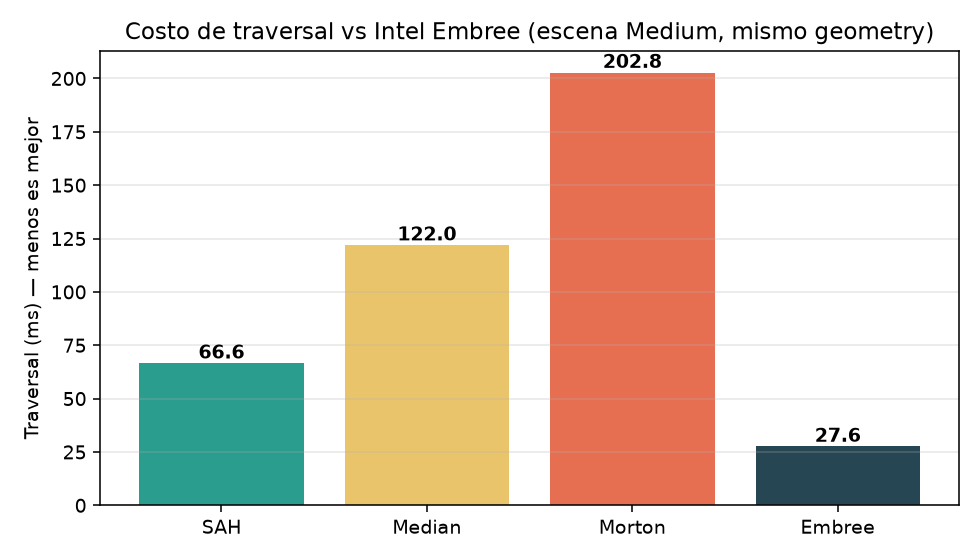
\includegraphics[width=\textwidth,height=0.72\textheight,keepaspectratio]{fig_embree.png}
\end{column}
\begin{column}{0.45\textwidth}
\begin{itemize}\itemsep3pt
  \item Misma geometr\'ia: Embree \hl{$\sim$33\,ms} vs nuestra SAH $\sim$79\,ms.
  \item \hl{$\sim$2{,}4$\times$} m\'as r\'apido.
  \item Embree = \emph{t\'ermino de comparaci\'on}, no competidor.
  \item Valida que estamos en el orden de magnitud correcto.
\end{itemize}
\end{column}
\end{columns}
\end{frame}

\begin{frame}{Escalado paralelo (m\'as benchmarks)}
\begin{columns}[T]
\begin{column}{0.6\textwidth}\centering
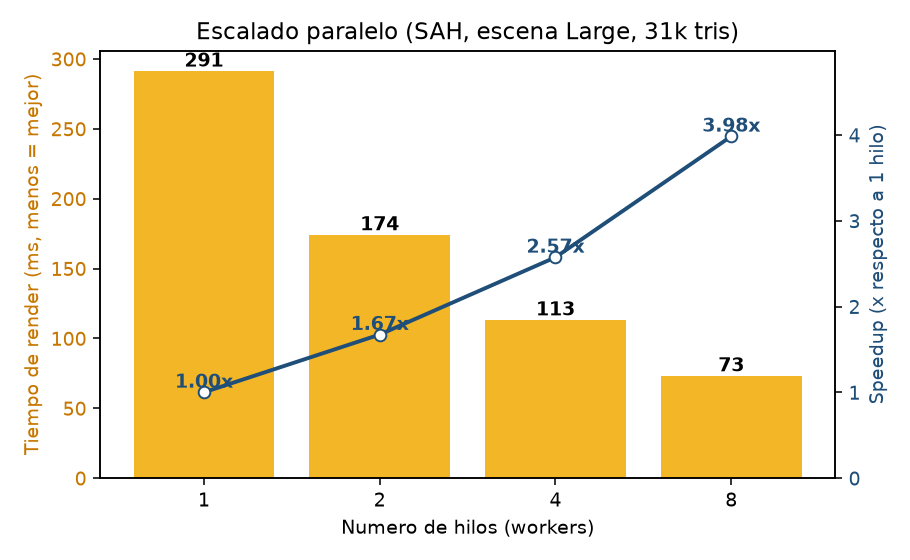
\includegraphics[width=\textwidth,height=0.72\textheight,keepaspectratio]{fig_speedup.png}
\end{column}
\begin{column}{0.4\textwidth}
\begin{itemize}\itemsep2pt
  \item SAH/Large, de 1 a 8 \emph{workers}.
  \item Render: \hl{291\,ms $\to$ 73\,ms}.
  \item \hl{Speedup $\sim$4$\times$} al usar los 10 n\'ucleos (4P+6E).
  \item El paralelismo por franjas escala muy bien.
\end{itemize}
\end{column}
\end{columns}
\end{frame}

%==============================================================================
\section{Conclusiones}
%==============================================================================

\begin{frame}{Conclusiones}
\begin{itemize}\itemsep4pt
  \item Ray tracer CPU completo con BVH y \hl{benchmark reproducible} (\texttt{-{}-bench}, \texttt{-{}-scaling}).
  \item Comparamos \hl{3 heur\'isticas} + referencia \hl{Embree} sobre la misma geometr\'ia.
  \item \hl{Hallazgo:} la \alert{SAH} da el mejor \'arbol ($\sim$3$\times$ menos nodos/rayo que Morton)
        $\Rightarrow$ render $\sim$3$\times$ m\'as r\'apido.
  \item La brecha con Embree est\'a en el \emph{recorrido SIMD} (MBVH), no en la estructura.
  \item El paralelismo por franjas escala $\sim$4$\times$ con los n\'ucleos disponibles.
\end{itemize}
\end{frame}

\begin{frame}{Demo en vivo}
\begin{center}
\begin{tikzpicture}
  \node[draw=prim,thick,rounded corners=4pt,fill=panel,minimum width=8cm,minimum height=3cm,align=center,text=ink] {%
    \Large \color{primdk}\bfseries Demo en tiempo real\\[6pt]
    \normalsize\color{ink} \texttt{./bvh\_raytracer --width 1280 --height 720}\\[4pt]
    \footnotesize\color{mute} TAB raytrace \textbullet{} B fuerza bruta \textbullet{} V cajas \textbullet{} M men\'u};
\end{tikzpicture}
\end{center}
\vspace{4pt}
\begin{itemize}
  \item Alternar SAH / Median / Morton en vivo y ver el cambio de FPS.
  \item Comparar BVH vs fuerza bruta $O(N)$ (tecla \texttt{B}).
  \item Visualizar las cajas del \'arbol (tecla \texttt{V}).
\end{itemize}
\end{frame}

\begin{frame}{Trabajo futuro}
\begin{columns}[T]
\begin{column}{0.5\textwidth}
\begin{itemize}\itemsep2pt
  \item Recorrido \hl{SIMD} (NEON): varios rayos/hijos por instrucci\'on.
  \item \hl{MBVH}: nodos de 4 v\'ias.
  \item Layout \hl{SoA} y nodos cuantizados.
\end{itemize}
\end{column}
\begin{column}{0.5\textwidth}
\begin{itemize}\itemsep2pt
  \item Construcci\'on \hl{paralela} del \'arbol.
  \item Comparar con \hl{SBVH} (split) para geometr\'ia que se intersecta.
  \item M\'as escenas y resoluciones.
\end{itemize}
\end{column}
\end{columns}
\end{frame}

%========================== GRACIAS ===========================================
\begin{frame}[plain,noframenumbering]
\begin{tikzpicture}[remember picture,overlay]
  \fill[prim] ([yshift=6mm]current page.south west) rectangle ([yshift=-6mm]current page.north west);
\end{tikzpicture}
\vfill\centering
{\color{primdk}\Huge\bfseries ¡Gracias!}\\[10pt]
{\color{ink}\Large Preguntas y respuestas}\\[18pt]
{\color{primdk}\rule{0.25\textwidth}{1.2pt}}\\[12pt]
{\color{mute}\small Ray tracing acelerado con BVH \textbullet{} UTEC \textbullet{} CS3014}
\vfill
\end{frame}

\end{document}
